\documentclass[final,5p,times,twocolumn]{elsarticle}

\usepackage{lineno}
\linenumbers

\begin{document}

\begin{frontmatter}

\title{Development of the CBM RICH readout electronics and DAQ}

\author[a]{J.~Adamczewski-Musch}
\author[h]{P.~Akishin}
\author[b]{K.-H.~Becker}
\author[h,f]{S.~Belogurov}
\author[d]{J.~Bendarouach}
\author[e]{N.~Boldyreva}
\author[d]{C.~Deveaux}
\author[e]{V.~Dobyrn}
\author[d]{M.~D\"urr}
%\author[f]{J.~Eom}
\author[a]{J.~Eschke}
\author[b]{J.~F\"ortsch}
\author[d]{J.~Heep}
\author[d]{C.~H\"ohne}
\author[b]{K.-H.~Kampert}
%\author[a]{V.~Kleipa} --?
\author[e,f]{L.~Kochenda}
%\author[a]{B.~Kolb} --?
\author[b,d]{J. Kopfer}
\author[e,f]{P.~Kravtsov}
\author[b]{I.~Kres}
\author[d,h]{S.~Lebedev}
\author[d]{E.~Lebedeva}
\author[e]{E.~Leonova}
\author[a]{S.~Linev}
\author[d]{T.~Mahmoud}
\author[g]{J.~Michel}
\author[e]{N.~Miftakhov}
%\author[f]{Y.~Nam}
\author[a]{W.~Niebur}
%\author[f]{K.~Oh}
\author[h,c]{E.~Ovcharenko\corref{cor1}} \ead{eovchar@jinr.ru}
\author[b]{V.~Patel}
\author[b]{C.~Pauly}
\author[b]{D.~Pfeifer}
%\author[b]{J.~Pouryamout}
\author[b]{S.~Querchfeld}
\author[b]{J.~Rautenberg}
\author[b]{S.~Reinecke}
\author[e]{Y.~Riabov}
\author[e]{E.~Roshchin}
\author[e,f,i]{V.~Samsonov}
\author[h,j]{V.~Schetinin}
%\author[f]{J.~Song}
\author[e]{O.~Tarasenkova}
%\author[a]{T.~Torres de Heidenreich} --?
\author[a]{M.~Traxler}
\author[a]{C.~Ugur}
\author[e]{E.~Vznuzdaev}
\author[e]{M.~Vznuzdaev}
%\author[f]{J.~Yi}
%\author[f]{I.-K.~Yoo}

\address[a]{GSI Helmholtzzentrum f\"ur Schwerionenforschung GmbH, D-64291 Darmstadt, Germany}
\address[b]{Department of Physics, University Wuppertal, D-42097 Wuppertal, Germany}
\address[c]{SSC RF Institute for Theoretical and Experimental Physics (ITEP), 117218 Moscow, Russia}
\address[d]{Institute of Physics II and Institute of Applied Physics, Justus Liebig University Giessen, D-35392 Giessen, Germany}
\address[e]{National Research Centre - Kurchatov Institute, B.~P.~Konstantinov Petersburg Nuclear Physics Institute, 188300 Gatchina, Russia}
%\address[f]{Department of Physics, Pusan National University, 609-735 Pusan, Republic of Korea}
\address[f]{National Research Nuclear University MEPhI (Moscow Engineering Physics Institute), 115409 Moscow, Russia}
\address[g]{Institut f{\"u}r Kernphysik, Goethe University Frankfurt, D-60438 Frankfurt am Main, Germany}
\address[h]{Laboratory of Information Technologies, Joint Institute for Nuclear Research (JINR-LIT), 141980 Dubna, Russia}
\address[i]{St.~Petersburg State Polytechnic University (SPbSPU), 195251 St.~Petersburg, Russia}
\address[j]{Bauman Moscow State Technical University, 105005 Moscow, Russia}

\cortext[cor1]{Corresponding author}

\begin{abstract}
A real size prototype of the CBM RICH detector was tested in beam at CERN in November 2014 with new readout electronics. A detailed analysis of the timing characteristics of the readout chain  will be presented in this article. Results of the time precision measurements for a subset of all channels and the stability of the fine time calibration will be discussed. The obtained sub-nanosecond time precision allows also to investigate the effect on timing when using additional wavelength-shifting films on top of the MAPMT windows.
\end{abstract}

\begin{keyword}
CBM; RICH; readout; DAQ; WLS; time precision.
\end{keyword}

\end{frontmatter}

%%%%%%%%%%%%%%%%%%%%%%%%%%%%%%%%%%%%%%%%%%%%%%%%%%%%%%%%%%%%%%%%%%%%%%%%%%%%%%%%%%%%%%%%%%%%%%%%%%%%%%%%%%%%%%%%

\section{Introduction}

The CBM experiment at the future FAIR facility (Darmstadt, Germany) will investigate strongly interacting matter at high net-baryon densities but moderate temperatures in heavy-ion collisions. The CBM RICH detector is required for identifying electrons in a momentum range up to 8~GeV/c \cite{CBMRICH1, CBMRICH2, CBMRICHPROJECT}. It is a classical RICH detector with gaseous radiator, spherical mirrors and segmented photosensitive camera made of approx. 1000~Hamamatsu H12700 multi-anode photomultiplier tubes (MAPMT). The MAPMTs will be read out by self-triggered FPGA-based front end boards (FEB) detecting only time information.

During common CBM beam tests at CERN-PS in Nov 2014 a CBM RICH prototype including a camera of 16~MAPMTs partially covered with p-terphenyl as wavelength shifter (WLS, \cite{WLS}) has been successfully tested. The MAPMTs were read out by 64~PADIWA FEBs and digitized by 64~TDCs located at 16~TRB~v3 boards \cite{TRB}. Further readout has been performed via two parallel chains: using FLES \cite{FLES} Interface Board (FLIB) and standard Ethernet via router to Network Interface Card (NIC). Figure~\ref{fig:BeamSetup} shows the scheme of the CBM RICH prototype during the beam tests.

\begin{figure}[h]
	\centering
	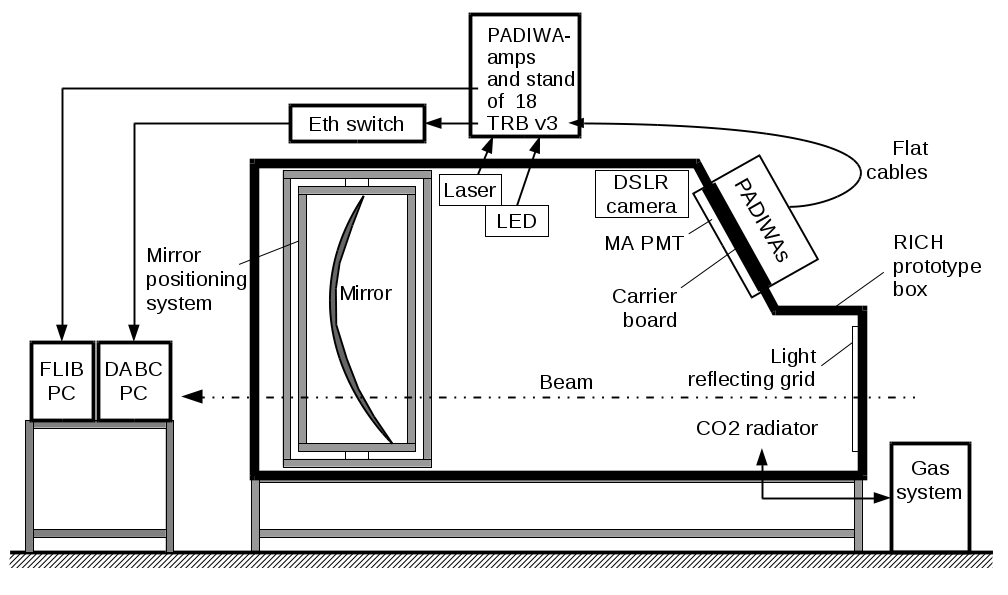
\includegraphics[width=0.48\textwidth]{figures/Beamtime_eng_RICH2016_poster.png}
	\caption{Sketch of the CBM RICH beam test setup.}
	\label{fig:BeamSetup}
\end{figure}

PADIWA is a 16~channel FEB which realizes a preamplifier and a discriminator with an adjustable threshold, the latter inside an FPGA. TRB~v3 is a multifunctional board which employs 5~FPGAs. The main TRB configuration used in CBM RICH has 4~peripheral FPGAs programmed as TDCs \cite{TDC} and 1~central FPGA programmed as HUB. One readout module (see \cite{PEPAN} for more details), consisting of 4~PADIWAs and 1~TRB, is used to read out one 64-pixel MAPMT. Timestamps of the leading and trailing edges of the discriminated signal are detected thus allowing the measurement of time-over-threshold (ToT).

The software for the CBM RICH data processing is implemented in the CbmRoot framework \cite{SEMEN}. All stages from readout to analysis can be performed «on the fly» with or without recording any intermediate information on disk. The data processing pipeline includes the following stages: unpacking, calibration, hit building, event building, reconstruction and analysis. See refs. \cite{PEPAN} and \cite{RINGS} for more details on the functionality and implementation.

%%%%%%%%%%%%%%%%%%%%%%%%%%%%%%%%%%%%%%%%%%%%%%%%%%%%%%%%%%%%%%%%%%%%%%%%%%%%%%%%%%%%%%%%%%%%%%%%%%%%%%%%%%%%%%%%

\section{Fine time calibration}

The detection of the timestamp in an FPGA-based TDC, used by CBM RICH, is done in two stages. The coarse time is registered using a circular counter which is controlled by the clock with a 5~ns period. The most significant 28~bits are called 'epoch' and the remaining 11~bits are called 'coarse time'. For more precise timestamp measurement an additional 10-bit register is used for a fine time value. The register is filled from the fine time counter implemented using Tapped Delay Line (TDL) on 512~elements. A calibration of the fine time is required to achieve best time precision. Using a small subset of the recorded data, for each channel a discrete calibration function $ f_{calib}(Fine) $ is built to translate the fine time counter value into the fine time in ns. The full time $ T $ in ns is then computed using the following formula:

{\centering
$ T = Epoch \cdot 2048 \cdot 5ns + Coarse \cdot 5ns - f_{calib}(Fine) $ \\
}

The non-linearity of the fine time dependence on the fine time counter value is presented in figure~\ref{fig:CalibTableMinusLinear}, where the difference between the extracted dependence to a linear dependence is shown. This difference does not exceed 150~ps. Figure~\ref{fig:CalibStability} shows the stability of this calibration with time comparing absolute time differences of fine time calibrations of three data subsets to the full data set. Here, different data subsets differ by a few minutes in data taking, the same stability is also observed for longer periods. Typical fluctuations are around 10~ps.

\begin{figure}[h]
	\centering
	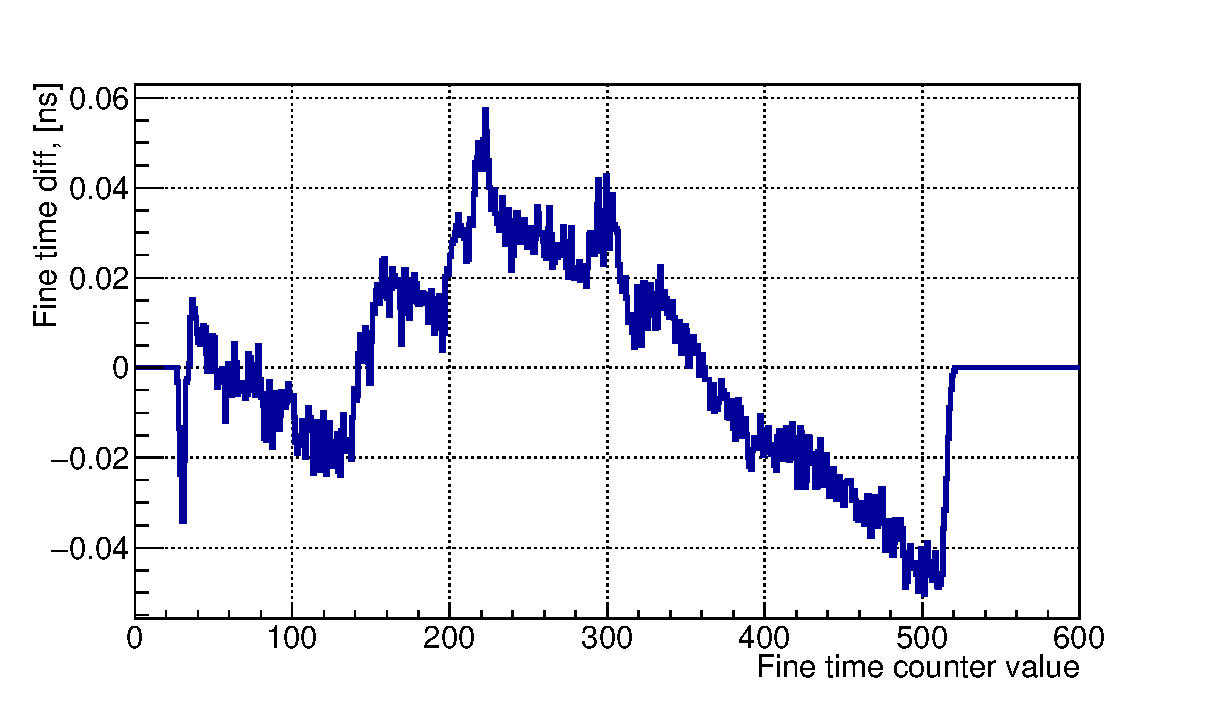
\includegraphics[width=0.48\textwidth]{figures/CalTableMinusFit_0010_01_feb2017.eps}
	\caption{Difference between the measured $ f_{calib} $ and assumed linear dependence of fine time vs. fine time counter value.}
	\label{fig:CalibTableMinusLinear}
\end{figure}

\begin{figure}[h]
	\centering
	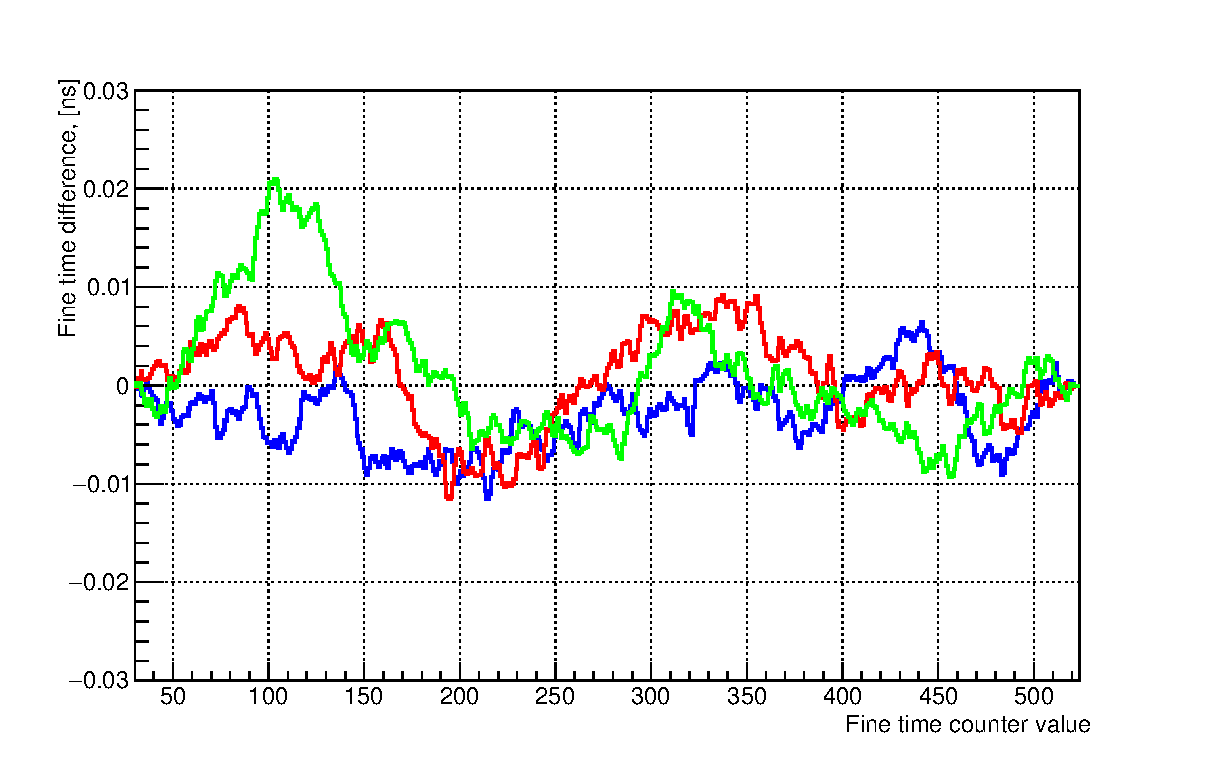
\includegraphics[width=0.48\textwidth]{figures/Stability_01_diff.eps}
	\caption{Stability of the calibration table comparing different data subsets.}
	\label{fig:CalibStability}
\end{figure}

%%%%%%%%%%%%%%%%%%%%%%%%%%%%%%%%%%%%%%%%%%%%%%%%%%%%%%%%%%%%%%%%%%%%%%%%%%%%%%%%%%%%%%%%%%%%%%%%%%%%%%%%%%%%%%%%

\section{Full readout chain time precision}

The data obtained during the CERN beam tests of the CBM RICH prototype have been used to determine the time resolution of the readout chain. A laser Alphalas Picopower LD405 coupled with the pulser Alphalas PLDD-250 \cite{LASER} was used as a source for fast ($<40ps$) light flashes. The analysis technique is based on the fact that signals in different channels within one event coming from one laser flash are simultaneous. Figure~\ref{fig:TimePrec} shows the time difference distributions of leading edge measurements for four different cases: comparing two channels (blue), comparing all 16~channels read out by one PADIWA FEB (red), comparing 64~channels from one MAPMT (green), and comparing the top-right quarter of the camera consisting of 4~MAPMTs (black). The distributions have been scaled to make the visual comparison easier. The FWHM and RMS values are listed in table~\ref{tabl:TimePrecTable}.

Increasing the number of channels under analysis the FWHM is increasing but the RMS stays almost the same. One can also observe that the shape of the distribution is approaching a Gaussian distribution. It means that peculiarities of individual channels are washed out by averaging. The reported FWHM values can be considered as $ \sqrt 2 $ times bigger than classically defined time precision because both terms of the time difference are fluctuating independently following similar distributions. Thus our estimation for the time precision is about 1.2~ns for the biggest analyzed subset of channels. This number exceeds the MAPMT transition time jitter and is dominated by the walk of the leading edge of the logical signal due to fluctuations of the single photoelectron amplitude. The walk corrections can be introduced if ToT is correctly measured. Unfortunately this was not possible in the current setup, see \cite{PEPAN} for details.

\begin{figure}[h]
	\centering
	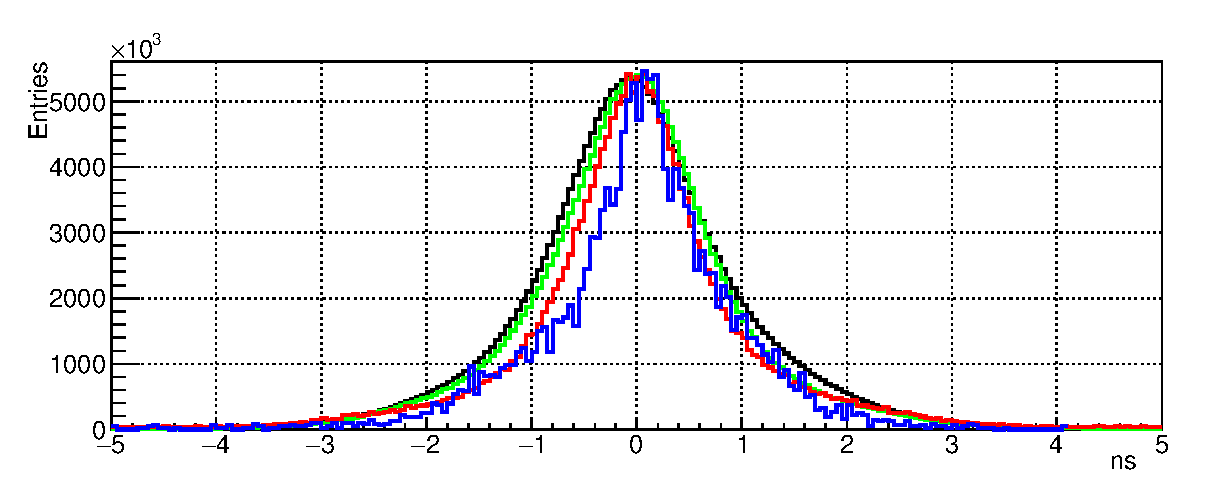
\includegraphics[width=0.5\textwidth]{figures/TimePrecision_evolution_noStats2.eps}
	\caption{The leading edge time difference distributions for different camera areas. Blue - one pair of channels; red - one PADIWA FEB; green - one MAPMT; black - 4 MAPMTs.}
	\label{fig:TimePrec}
\end{figure}

\begin{table}[h]
\centering
	\begin{tabular}{ | p{0.22\linewidth} | p{0.10\linewidth} | p{0.10\linewidth} | p{0.12\linewidth} | p{0.12\linewidth} | }
		\hline		
		\scriptsize{Analyzed area} & \scriptsize{A pair of channels} & \scriptsize{One PADIWA} & \scriptsize{One MAPMT} & \scriptsize{Camera quarter} \\
		\hline
		\scriptsize{Num. of channels} & 2 & 16 & 64 & 256\\
		\hline
		\scriptsize{FWHM, ns} & 1.00 & 1.22 & 1.50 & 1.64\\
		\hline
		\scriptsize{RMS, ns} & 0.912 & 1.093 & 0.996 & 1.034\\
		\hline
	\end{tabular}

	\caption{FWHM and RMS of the leading edge time difference distributions for different analyzed areas.}
	\label{tabl:TimePrecTable}

\end{table}

%%%%%%%%%%%%%%%%%%%%%%%%%%%%%%%%%%%%%%%%%%%%%%%%%%%%%%%%%%%%%%%%%%%%%%%%%%%%%%%%%%%%%%%%%%%%%%%%%%%%%%%%%%%%%%%%

\section{p-terphenyl WLS effect on timing}

During RICH prototype beam test effects due to the WLS coating were studied. There were 3 groups of MAPMTs in the camera: (1)~covered with WLS layers for the first runs, then cleaned and used without WLS films for the second set of runs, (2)~covered with WLS layers for the whole beamtime and (3)~not covered for the whole beamtime. By comparison of the data received using the MAPMTs from the first group~(1) we can analyse the effect of WLS layers.

Beam events may contain Cherenkov rings on the camera plane. The photons belonging to each detected Cherenkov ring can be considered as simultaneous. In each event, i.e. the Cherenkov ring, the first hit in time is used to define the reference time $ t_{ref} $. For all other hits in the event, the time difference, $ \Delta t_i = t_i - t_{ref} $, $ i \neq ref $ is computed.

An exponential fit with one component to the timing distribution without WLS layer in figure~\ref{fig:WLS} (blue) yields a decay constant of 540~ps. Fixing this and performing a three-exponential fit to the remaining WLS layer contribution (fig.~\ref{fig:WLSdiff}) three decay constants are observed:
\begin{center}
\begin{tabular}{ c c c }
$ \tau_1 = 1.4 ns $, & $ \tau_2 = 3.8 ns $, & $ \tau_3 = 45 ns $. \\
\end{tabular}
\end{center}
The fast component comprises about 80\% of all WLS hits. This timing profile extracted from data analysis agrees very well with independent additional time-dependent fluorescence measurements from a spectrometer.
Within a coincidence window of 20~ns 95\% of all hits can be collected when applying WLS layers. Depending on interaction rates such timing windows are well feasible for the CBM RICH and thus allow to use WLS layers for increased UV sensitivity of the photodetector.

\begin{figure}[h]
	\centering
	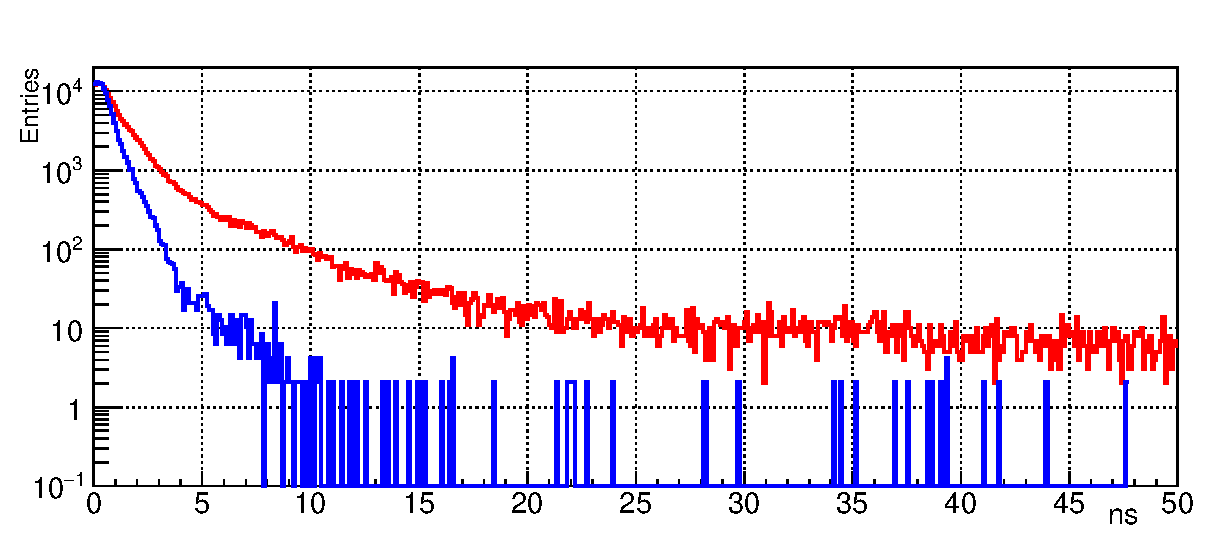
\includegraphics[width=0.48\textwidth]{figures/Two_curves_1Nov.eps}
	\caption{Time difference distribution of all hits within one Cherenkov ring without (blue) and with (red) WLS layer application.}
	\label{fig:WLS}
\end{figure}

\begin{figure}[h]
	\centering
	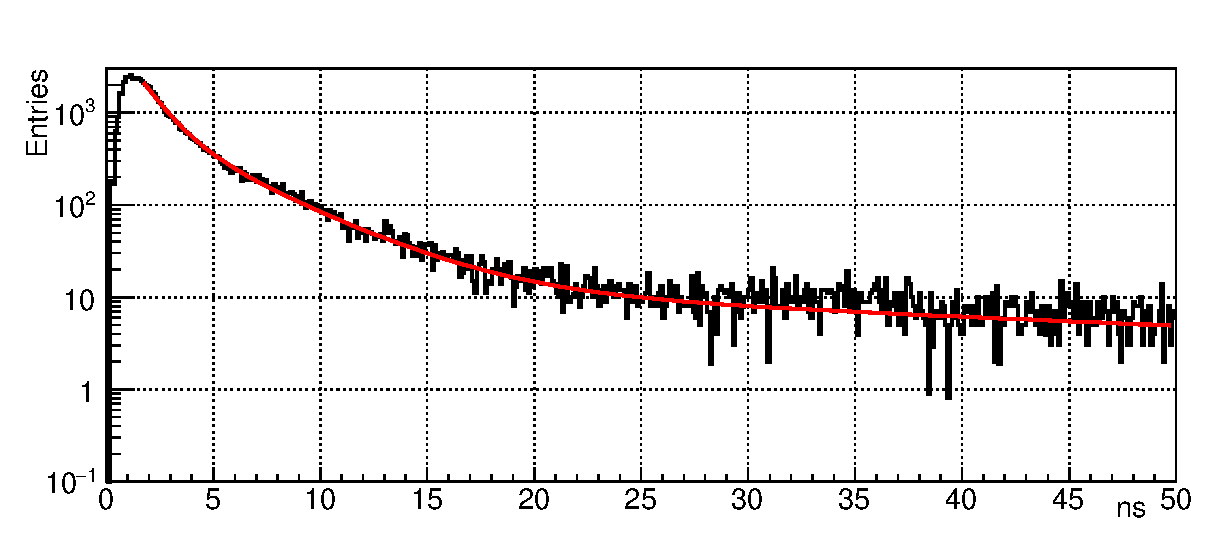
\includegraphics[width=0.48\textwidth]{figures/WLSdiff_1Nov.eps}
	\caption{Time profile of Cherenkov hits from WLS layer: difference of timing distributions shown in figure \ref{fig:WLS}. The red line shows the fit result presented in the text.}
	\label{fig:WLSdiff}
\end{figure}

%%%%%%%%%%%%%%%%%%%%%%%%%%%%%%%%%%%%%%%%%%%%%%%%%%%%%%%%%%%%%%%%%%%%%%%%%%%%%%%%%%%%%%%%%%%%%%%%%%%%%%%%%%%%%%%%\\

\section{Summary}

The timing performance of the readout system prototype of the CBM RICH detector has been investigated. In this article effects due to (a) wave-length shifting films, (b) transition time spread within one readout board, one MAPMT and for several MAPMTs, and (c) accuracy and stability of the TDC calibration are demonstrated and discussed. The detailed analysis of the readout electronics as presented here led to improvements implemented in the next iteration of the RICH readout which is presented in \cite{PAULY}.

%%%%%%%%%%%%%%%%%%%%%%%%%%%%%%%%%%%%%%%%%%%%%%%%%%%%%%%%%%%%%%%%%%%%%%%%%%%%%%%%%%%%%%%%%%%%%%%%%%%%%%%%%%%%%%%%

\section*{Acknowledgements}

This work was supported by the Hessian LOEWE initiative through the Helmholtz International Center for FAIR (HIC for FAIR), by the Helmholtz Graduate School for Hadron and Ion Research, by the GSI F\&E-Cooperation with Giessen and Wuppertal (WKAMPE1012), by BMBF Grants 05P12RGFCG, 05P12PXFCE, 05P09PXFC5, 05P15PXFCA and 05P15RGFCA, by Helmholtz Grant IK-RU-002, by SC~ROSATOM through FRRC, and by the Ministry of Education and Science of the Russian Federation (grant no. 14.A12.31.0002) in accordance with the Russian Federation Government Regulation no. 220.

%%%%%%%%%%%%%%%%%%%%%%%%%%%%%%%%%%%%%%%%%%%%%%%%%%%%%%%%%%%%%%%%%%%%%%%%%%%%%%%%%%%%%%%%%%%%%%%%%%%%%%%%%%%%%%%%

\section*{References}

\begin{thebibliography}{99}

\bibitem{CBMRICH1}
C.~Hoehne, et. al.,
%Development of a RICH detector for electron identification in CBM,
NIM A 595 (2008) 187

\bibitem{CBMRICH2}
C.~Hoehne, et. al.,
%Development of a RICH detector for CBM: simulations and experimental tests,
NIM A 639 (2011) 294

\bibitem{CBMRICHPROJECT}
J. Adamczewski-Musch, et al.,
%The CBM RICH project,
NIM A 766 (2014) 101

\bibitem{WLS}
J. Adamczewski-Musch, et. al.,
%Influence of wavelength-shifting films on multianode PMTs with UV-extended windows,
NIM A 783 (2015) 43

\bibitem{TRB}
A Neiser et al 2013 JINST 8 C12043
%A. Neiser, et. al.,
%TRB3: a 264 channel high precision TDC platform and its applications,
%2013 JINST 8 C12043

\bibitem{FLES}
J de Cuveland et al 2011 J. Phys.: Conf. Ser. 331 022006
%A First-level Event Selector for the CBM Experiment at FAIR,
%J. de Cuveland, V. Lindenstruth (for the CBM Collaboration)
%2011 J. Phys.: Conf. Ser. 331 022006

\bibitem{TDC}
C. Ugur, et. al.,
264 Channel TDC Platform Applying 65 Channel High Precision (7.2 ps RMS) FPGA Based TDCs,
10.1109/NoMeTDC.2013.6658234

\bibitem{PEPAN}
J. Adamczewski-Musch, et. al.,
Tests of the CBM RICH readout and DAQ prototype,
submitted to 'PEPAN leters'

\bibitem{SEMEN}
S.~Lebedev,
this issue

\bibitem{RINGS}
S Lebedev et al 2010 J. Phys.: Conf. Ser. 219 032015 
%S. Lebedev, C. Hohne, G. Ososkov,
%Ring Recognition and Electron Identication in the RICH detector of the CBM Experiment at FAIR,
%2010 J. Phys.: Conf. Ser. Vol. 219 032015,
%10.1088/1742-6596/219/3/032015

\bibitem{LASER}
Laser and pulser official site,
http://www.alphalas.com/products/lasers/ picosecond-pulse-diode-lasers-with-driver-picopower-ld-series.html

\bibitem{PAULY}
C.~Pauly,
this issue

\end{thebibliography}

%%%%%%%%%%%%%%%%%%%%%%%%%%%%%%%%%%%%%%%%%%%%%%%%%%%%%%%%%%%%%%%%%%%%%%%%%%%%%%%%%%%%%%%%%%%%%%%%%%%%%%%%%%%%%%%%

\end{document}